\myChapter{A methodology for developing services for EAs}\label{chap:soaea}


\begin{flushright}{\slshape
    I don't claim to be a methodologist, but I act like one only because
     I do methodology to protect myself from crazy methodologists. } \\ \medskip
    --- {Ward Cunningham (2004) Geek Noise}
\end{flushright}

\minitoc\mtcskip
\vfill
\lettrine{S}{OA} provides a good set of solutions to solve some of the
problems in the EA area, such as the lack of integration,
standardization and dynamism control, as presented in Section \ref{chap:distributed:conclusiones}. It also allows ease of
development in dynamic, distributed and heterogeneous systems, like the ones presented in Section \ref{chap:distributed:newtrendson}. % ¿quién
                                % ha dicho que eso es un problema? - JJ FERGU: ENLAZADO

 %However, several restrictions must be taken into account. In this
 %chapter, we present the existent restrictions in the EA design,
 %according to \person{Gagn\'e and Parizeau} \cite{GENERICITY05}. Also,
 %the restrictions in SOA design (such as the unordered execution or
 %distribution transparency) are explained to perform % are explained
                                % to perform? - Jj FERGU: BORRADO
 %a good design of services for EAs. All these requirements are used to explain how the different elements of an EA must be designed. % cita el capítulo anterior - JJ FERGU: Done

SOMA methodology, explained in previous chapter (Section \ref{chap:soa:methodologies}), establishes that the phases of the SOA design are {\em identification}, {\em specification}, {\em implementation} and {\em deployment} of the services and flows. Although SOMA is more focused in business environments (therefore other phases exist), the ideas that it offers are used to develop a methodology for the design of services for EAs. In this chapter the SOA-EA methodology is presented. SOA-EA is an abstract methodology to develop \textsc{service oriented evolutionary algorithms} (SOEAs), that is, evolutionary algorithms whose elements are services, independently of the technology to be used. It is formed by several phases to identify the services that compose an EA and specify some of their possible behaviours, taking into account the restrictions presented in Section \ref{sec:soa:restrictions}. The implementation and deployment of the designed services will be explained, using an specific technology, in the next chapter.

% Pon siempre en relación con la TESIS - JJ

%For a better understanding, a complete example of development of an EA
%is explained. This example is modified to show how to convert an
%algorithm to another, dynamic operator changing, load balancing and
%even intelligent aggregation of operators. 

% ¿Este capítulo es ciencia? ¿Tecnología? ¿Puro desarrollo? Deja bien
% clara la aportación de este artículo, aparte de la obvia
% implementación. ¿Has hecho una abstracción de los algoritmos
% genéticos? ¿Un survey de técnicas usadas? - JJ FERGU: Reescribiendo ENTERO el capítulo


%FERGU: he movido la sección que había aquí al capítulo anterior

%FERGU: TODO poner el problema a resolver


\section{Steps for designing services for EAs}
\lettrine{T}{his} section presents all the steps to design and implement services for Evolutionary Algorithms.
 As in SOMA, the phases are not linear, but they are iterative and incremental, that is, the designer can move back to a previous step if necessary. For example,
 new services can be discovered during the specification phase or changes on the specification could appear in the deployment phase. Figure \ref{fig:distributed:methodology} shows the steps of the proposed methodology.

\begin{SCfigure}[20][htb]
\centering
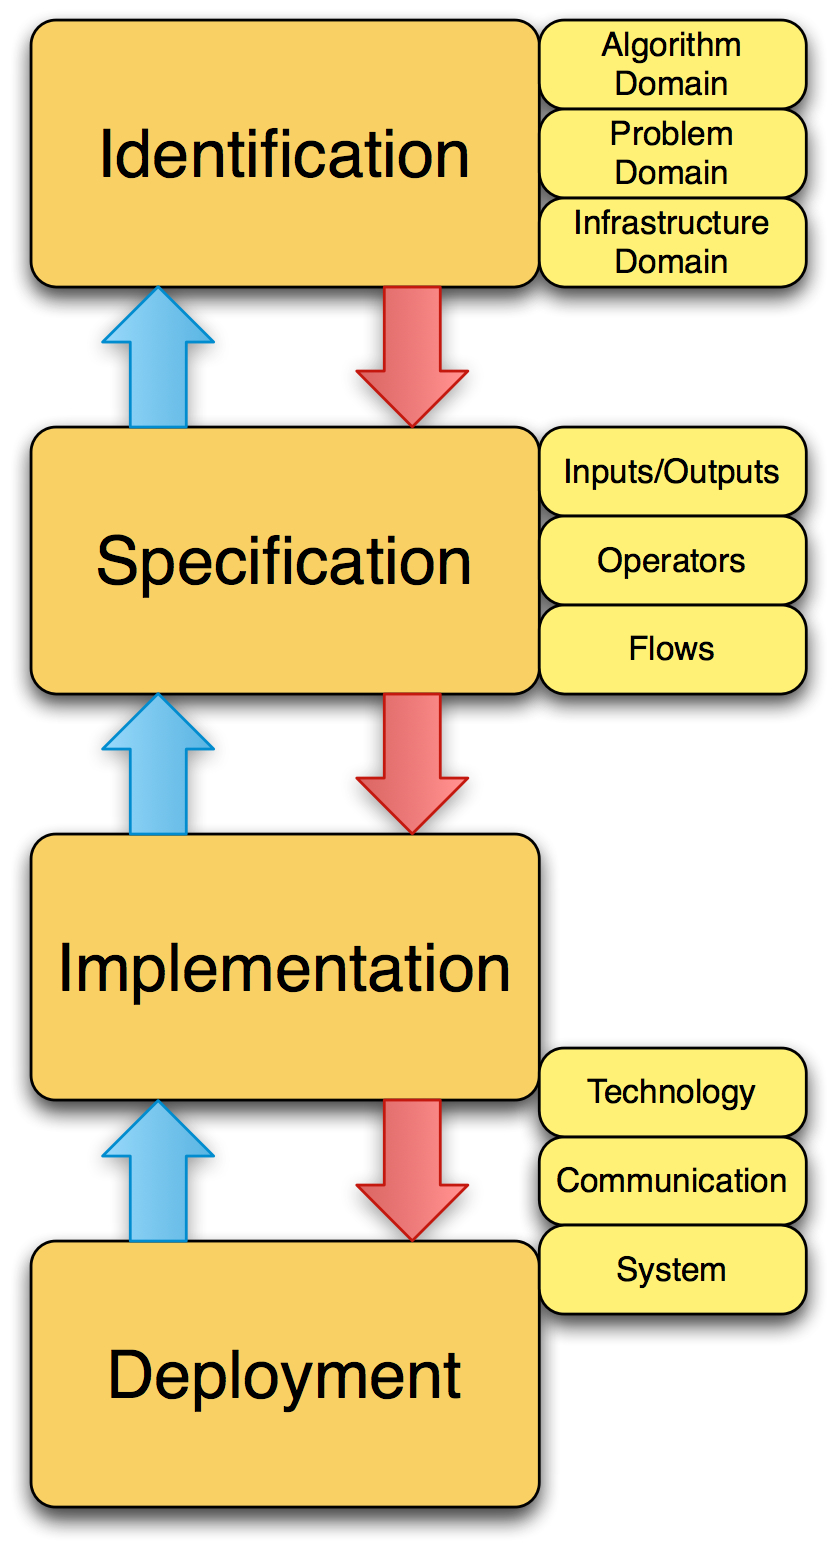
\includegraphics[width=5cm]{gfx/soaea/methodology.jpg}
\caption{Methodology to develop services for Evolutionary Algorithms.}
\label{fig:distributed:methodology}
\end{SCfigure}

\section{Identification}
\label{subsec:soaea:identification}

\lettrine{T}{his} phase is focused on the identification of the three constructs of SOA: services, components and flows. So, at the end of this step, the developers have a complete list of the services to be designed.

First, the developers should ask themselves the following questions to facilitate the identification:
\begin{itemize}
\item Which problem do I need to solve?
\item What elements are needed my EA?
\item Has somebody else programmed this before?
\item Which operators do I need?
\item Is my algorithm going to be extended in the future?
\item How can I parametrize my algorithm?
\end{itemize}

Solving the previous questions is the first step to identify the services. The next step is to classify the services in one of the three different domains that are proposed: {\em Algorithm domain}, the {\em Problem Domain} and the {\em Infrastructure Domain}. 

\subsection{Algorithm domain} Services in this domain are those that conform the EA. For example, operators of individuals, stop criterion, or populations.
 Also, getting the values of the parameters can also be a
  service,  thus the EA developer obtains two advantages over using parameters only as variables: 
it is not mandatory to distribute the parameters among all services, and also they can be dynamically modified in execution time from an external service, facilitating self-adaptation.

\subsection{Problem domain} In this domain, the user defines the services to address the elements of the problem. An example is the fitness function. The fitness function is a clear EA element that can be designed as a service. Each problem should implement an interface
  of the fitness service that receives the individual, allowing the
  distribution of this service (instead of being a method in the {\em individual} class, for example). There are also other services that depend on the problem, such as an initializer of individuals.

\subsection{Infrastructure domain} Services in this domain are the ones that deal with the specific infrastructure that will be used to execute the algorithm. For example, services for user control, load balancing or logging. The design of many of these services is out of the scope of the EAs, but all them have to interact with the previous domains in some way. Depending on the environment where the EA is going to be developed, other services need to be modelled. For example, user control in cloud environments, different mechanisms for logging (in console, GUI...) or interconnection with other systems (such as external databases).

 

\section{Specification}

\lettrine{O}{nce} the services have been identified, the next step of the methodology establishes the inputs and outputs of the services. The questions to solve prior to this phase are:

\begin{itemize}
\item Which are the inputs of the services?
\item Which are the operations of each service?
\item How are the services going to be used?
\item Which is the order of execution of the services?
\item Is only one type of service required?
\end{itemize}

All the characteristics of genericity for the design of an EAs, presented in Section \ref{sec:distributed:design}, should be taken into account when designing elements for EAs. However, requirements are also aligned with the requirements for designing services, explained in previous chapter (Section \ref{sec:soa:restrictions}). It is important to remark that in the future these services could be extended, so they should be designed taking into account this possibility.



\subsection{Specifying the operators}
When specifying operators (such as 
{\em recombinator} or {\em mutator}) they do not have to be modelled to receive one or two
individuals, since not all EAs have the same behaviour. They should receive a
list of individuals to be crossed or mutated each generation. Almost all services in an EA (like {\em mutation} or {\em selection}) will accept individuals as input data and produce/modify these individuals. Due to many kind of individuals may exist, the operators should be as abstract as possible to work properly. Therefore, services must accept interfaces of individuals as inputs, not concrete implementations, such as vectors or lists (generic representation). 

\subsection{Specifying the population} The population should not be a list of individuals: it should be a service
to access the individuals and allow the variation of its structure (for example, a change
from an unique list population to a cellular model) without
affecting  the rest of the services of the algorithm. So, other services
external to the EA could consult the {\em population} state and act
accordingly to some rules. 

\subsection{Specifying the fitness}
As previously stated in Section \ref{sec:soa:restrictions}, % ¿dónde? ¿Para qué están los hiperenlaces? - JJ FERGU: Añadido As in the operators, 
 the fitness should not be calculated within a method of an {\em Individual} class. To be less
coupled, it should be implemented as an external service that receives a list of individuals (facilitating the load balancing). That way, the service is as abstract as possible. 
%However, to be more flexible, the {\em fitness service} must receive a list of at least one individual, to facilitate the parallelism (and also to accomplish the generic fitness restrictions in design for EAs). % ¿Seguro que hace falta
                                % esto? ¿No hará falta un simple
                                % servicio de selección? Tienes que
                                % justificarlo todo sobre todo si es
                                % parte de TU TESIS - JJ FERGU: Comentado eso, que se me ha escapado

\subsection{Specifying the parameters}
The parameter set should be a service for the same reason, allowing the possibility of performing
experiments related to  parameter control or tuning \cite{ParameterControlEiben07} in an efficient way
(being separated from the code of the existing operators). 

\subsection{Specifying the flow of the services}

A SOEA can be seen as a service flow. Flows should be designed to reduce the impact of potential future changes. An example of service flow would be an implementation called {\em Evolutionary Algorithm} with all the steps common to all EAs and with independence of the implementations of these steps (generic evolutionary model). This allow the adaptation of the evolutionary model. The user can manually
  select the services to be combined to create a Genetic Algorithm or
  an Evolution Strategy, for example.  


  Furthermore, to accomplish with the genericity presented in Section \ref{sec:distributed:design}, the parameters and operators should be added dynamically. This is done with the SOA service binding. Users can specify the operators they need in several ways, for example, in a configuration file, or in an intelligent manner (an algorithm), taking into account the classification about evidence in parameter control presented in Section \ref{chap:distributed:parameteradapt} . It is important to remark that these ``pieces'' do not need to be modified and compiled again, because the loose coupling and the dynamic binding of SOA. Without SOA this behaviour is very difficult to achieve or maintain, as will be explained in next section.

\subsection{Specifying the infrastructure services}
The infrastructure services function is to manage the system. For example, output mechanisms (GUI or logging services) that should be independent of the services of the other domains. In this step, also the control of the system should be described (for example, user control or load balancing control).





%Definition or addition of every type of operator. % ¿definition
                                % or addition? - JJ FERGU: BORRADO



%Thanks to the loose coupling of services, several crossover or
%mutation implementations can be created. % esto no haces más que
                                % repetirlo. Pero ¿lo has hecho? Si
                                % usas servicios web por esto, tienes
                                % que usarlo en la tesis (y además te
                                % lo llevo diciendo casi desde que
                                % empezaste con este tema) - JJ FERGU: BORRADO, y sí, lo hago.
%Moreover, new operators can be added in execution time, without
%re-compiling the existing ones, or combining them according to several
%parameters, for example. % pero ¿esto lo vas a hacer? Recuerda el
                         % principio de espada del samurai: si la
                         % desenvainas, tiene que hacer sangre; si
                         % hablas de esto, tienes que usarlo (aunque
                         % sea como prueba de concepto)- JJ FERGU: sí, lo hago




%hala, repitiendo lo que dices en el capítulo anterior. Pa matarte. - JJ FERGU: borrado el párrafo entero



\section{Implementation and deployment}
\label{subsec:soaea:implementation}
\lettrine{O}{nce} the services have been identified and specified, a SOA technology should be used to implement and publish them. These two steps of the methodology are explained together because the decisions about the technological solution to be used is bound to both phases.

The questions to solve in these steps are:
\begin{itemize}
\item Are services going to be used locally or remotely?
\item How the interfaces are going to be exposed?
\item Are the services public?
\item How are going the changes in service dynamism to be managed?
\item How must be the overload of the messages? 
\item Which are the advantages of the chosen technology?
\item Which are the specific considerations about security, persistence, benchmarking and monitoring?
\end{itemize} 

\subsection{Select the technology to expose the interface}
As presented in Section \ref{chap:soa:implementations}, there exist several technologies to implement services. Depending on the use of the services, one technology should be chosen over other. For example, a service that is going to be used remotely and publicly from any programming language should export its interface with WSDL publicly available with an URL, to allow users to automatically generate the client for that service. On the other side, interfaces could be previously known, and it is not necessary to export them to the public. This is the case of OSGi, where the interface is exposed only to the OSGi service registry. Other mechanisms could be used to publish and share the interfaces of the services (for example, using a {\em newcast} protocol).

\subsection{Select the communication mechanism}
Services are also independent of the transmission mechanism, so this issue must be considered depending on the system to deploy the services. In the case of EAs, where the performance is important, usually the most efficient transmission mechanism should be preferred. However, sometimes other transmission mechanism can be used. For example, SOAP (explained in Section \ref{chap:soa:implementations}), includes extra information in headers \cite{Castillo13SOAP}, producing more network overload. However, this information is easier to manage for other systems, or easier to configure to be used remotely (as it uses a standard HTTP port).

\subsection{Deploy in the system} 
Once the services have been implemented they have to be deployed in the desired system. Examples of environment to deploy services are application servers (such as Apache Tomcat or Oracle GlassFish), service containers (Equinox or Felix), BPEL engines (for example OpenESB) or as a stand-alone system. In this step, issues related with testing, user control, security and persistence should be taken into account. The implementations of the infrastructure services deal with the chosen system.




%Taking into account the previous restrictions a possible way for designing services for EAs is shown: 
% ¿Esto es algo de tu tesis? Haz más énfasis y di cómo has llegado a esa forma "posible". ¿Es la única forma? ¿Es la mejor? ¿Qué otras has probado¿ -JJ
% FERGU: reestructurado el capítulo y explicada la metodología








\section{Conclusions}

\lettrine{C}{hapter} \ref{chap:distributedEAs} presented several shortcomings in the Evolutionary Algorithms area, such as the  incompatibility between frameworks or how to handle with new trends of distributed programming, where nodes enter and exit in runtime, for example. All these facts  motivate the creation of a proper way to define service oriented evolutionary algorithms (SOEAs) to facilitate the development, integration, standardization and dynamism.

In this chapter the requirements in EA design (genericity in representation, fitness, operations, model, parameters and output) presented  in Section \ref{sec:distributed:design}, with the requirements in SOA (genericity in interfaces, language independence, distribution and dynamism) explained in Section \ref{sec:soa:restrictions}, have been taken into account to propose a methodology to model the services that compose a service oriented EA, and several guidelines about the design of these services have been explained. This methodology proposes 4 iteratively and incremental phases: identification, specification, implementation and deployment. A number of questions has been proposed to answer in each phase to help in the development. This methodology can been used to create a service-oriented evolutionary algorithm that takes advantage of the SOA capabilities, such as loose-coupled services and automatic binding of new operators. 



Table \ref{tab:reasons} shows the advantages to design the elements of the EA as services.

\begin{SCtable}[][t]

\resizebox{11cm}{!}{
\begin{tabular}{p{2cm}p{2.5cm}p{3cm}p{7cm}}
%\begin{tabular}{llll}
%\noalign{\smallskip}\hline\noalign{\smallskip}
\hline
\rowcolor{colorCorporativoSuave}\textbf{Element} & \textbf{Current EAs development} & \textbf{Using SOA} & \textbf{Reason to migrate} \\
\hline \hline
%\rowcolor{colorCorporativoMasSuave}\noalign{\smallskip}\hline\noalign{\smallskip}
\rowcolor{colorCorporativoMasSuave}{\em Programming language} & Just one for all elements of the algorithm & Any & Services are independent of the programming language. Only the interface is required to use services  \\\hline
\rowcolor{colorCorporativoSuave}{\em Operators} & Methods or functions & Services & Services allow the selection of a specific implementation during the algorithm execution, and also different programming languages or distribution models\\\hline
\rowcolor{colorCorporativoMasSuave}{\em Operators behaviour} & Methods applied to a single individual & Service that receive individual lists  & It allows  load balancing and distribution, and also to modify the operators in execution time\\\hline
\rowcolor{colorCorporativoSuave}{\em Operator selection} & Modifying the source code & In a flexible way outside the source code & It is not mandatory to recompile the source code to integrate new operators \\\hline
\rowcolor{colorCorporativoMasSuave}{\em Fitness} & Method that evaluates an individual & Service that evaluates an individual list & It allows the distribution, load balancing and addition of new fitness calculators in real time \\\hline
\rowcolor{colorCorporativoSuave}{\em Population} & Array or individual list & Population service & It allows to change the population type and topography, by selecting the service implementation \\\hline
\rowcolor{colorCorporativoMasSuave}{\em Self-adaptation} & Modifying source code for a specific experiment & Self-adapting service that selects specific operator implementations & It does not modify the created services and brings more flexibility in the dynamic adaptation \\\hline
\rowcolor{colorCorporativoSuave}{\em Distribution} & Libraries like MPI & SOA mechanisms & SOA technologies allow changing the transmission protocol and using extra technologies without adding extra code\\
%\noalign{\smallskip}\hline
\hline
\end{tabular}
}
\caption{Summary of migration from traditional EA programming to SOA}

\label{tab:reasons}
\end{SCtable}

Next chapter will present a complete example of development and will explain how to modify services to change from a model to another, adding transparent distribution and load-balancing or dynamic adaptation of the parameters.



